\chapter{\MakeUppercase{Methodology and Testing}}

Example figures
\begin{figure}[h]
    \centering
    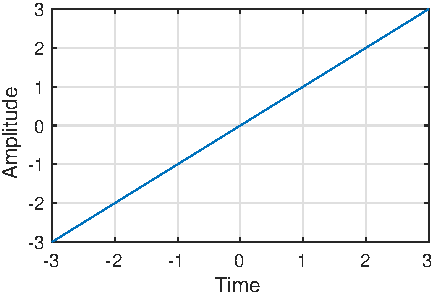
\includegraphics[width=0.5\linewidth]{images/sample-graph.pdf}
    \caption{Graph with straight line}
    \label{fig:universe}
\end{figure}
\begin{figure}[h!]
    \centering
    % Left image (a)
    \begin{subfigure}[b]{0.45\linewidth}
        \centering
        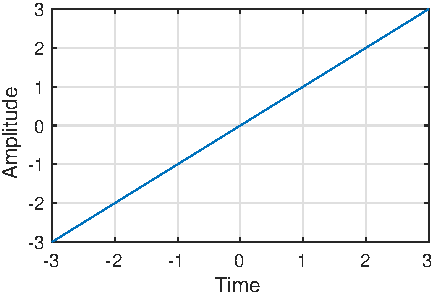
\includegraphics[width=\textwidth]{images/sample-graph.pdf} % replace with your image filename
        \caption{Graph-1}
        \label{fig:fruitsA}
    \end{subfigure}
    \hfill
    % Right image (b)
    \begin{subfigure}[b]{0.45\linewidth}
        \centering
        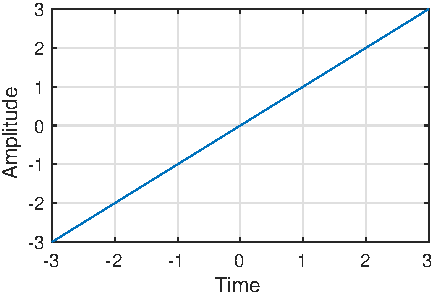
\includegraphics[width=\textwidth]{images/sample-graph.pdf} % replace with your image filename
        \caption{Graph-2}
        \label{fig:fruitsC}
    \end{subfigure}
    
    \caption{Two figures arranged side-by-side}
    \label{fig:common_fruits}
\end{figure}